
% \begin{frame}
% \frametitle{Aim: Estimate the progression of Alzheimer's disease}
% 
% Estimate the progression of Alzheimer's disease 
% 
% 
% 
% \end{frame}

\section{Disease Progression Modelling}

\begin{frame}
\frametitle{Alzheimer's Disease is a Devastating Disease}

\vspace{-1em}
\begin{itemize}
 \item 46 million people affected worldwide
 
  \begin{figure}
 \centering
%   \includegraphics[height=3cm]{adPrelavence}
  \includegraphics[height=4cm]{adPrevalanceIncreasing}
 \end{figure}
 
 \onslide<2-> \item No treatments available that stop or slow down cognitive decline
 \onslide<2-> \item Q: Why did clinical trials fail? A: Treatments were not administered early enough 
 \vspace{1em}
 \onslide<3-> \item Q: How can we then identify subjects \textbf{early} in order to administer treatments? 
 \onslide<3-> \item A: Disease progression model ...
 

\end{itemize}

\vspace{-1em}

\end{frame}

\newcommand{\sz}{1}

\begin{frame}{Building a Disease Progression Model}

\begin{columns}
\begin{column}{0.80\textwidth}
 
% \vspace{-2em}
\begin{center}
\begin{overprint}
\onslide<1> \incw{dps_series9}{\sz}
\onslide<2> \incw{dps_series8}{\sz}
\onslide<3> \incw{dps_series7}{\sz}
\onslide<4> \incw{dps_series6}{\sz}
\onslide<5> \incw{dps_series5}{\sz}
\onslide<6> \incw{dps_series4}{\sz}
\onslide<7> \incw{dps_series3}{\sz}
\onslide<8> \incw{dps_series2}{\sz}
\onslide<9> \incw{dps_series1}{\sz}
\onslide<10-> \incw{dps_series0}{\sz}
\end{overprint}
\end{center}

\begin{itemize}
\onslide<11-> \item Can now build population model
\onslide<12-> \item Early diagnosis
\end{itemize}
\end{column}
\begin{column}[t]{0.2\textwidth}
\vspace{-8em}

\onslide<13-> Previous models:
\onslide<13-> \begin{itemize}
 \item Jedynak, 2012
 \item Fontejin, 2012 
 \item Donohue, 2014
 \item Schiratti, 2017
 \item Lorenzi, 2019
\end{itemize}

\vspace{2em}

\onslide<14-> Limitation: require brain segmentation a-priori

\end{column}


\end{columns}



\end{frame}



% \begin{frame}
% \frametitle{Previous Disease Progression Models required Brain Segmentation ``a-priori''}
% 
% \newcommand{\mnpHeight}{3cm}
% 
% \vspace{-3em}
% % \textbf{Background}:
% \begin{itemize}
% %   \item Modelling the progression of Alzheimer's disease can potentially help drug development
%  \item Several data-driven disease progression models have been recently formulated:
%  
% %   \vfill 
%  
%  \hspace{-2em}
%  \begin{small}
%  \begin{figure}[h]
%  \centering
% %    \begin{minipage}[t][\mnpHeight][t]{0.49\linewidth}
% %   \centering
% %    \textbf{Event-Based Model}\\ 
% %    \begin{subfigure}{0.57\textwidth}
% %    \vspace{-6em}
% %    \includegraphics[width=\textwidth,trim=0 0 450 0,clip]{young_progression2}
% %    
% % %     \includegraphics[width=\textwidth,trim=450 0 0 0,clip]{young_progression2} 
% %    \end{subfigure}
% % %     \vspace{1em}
% %    \includegraphics[width=0.4\textwidth]{young_positional_variance}
% %   \end{minipage}
%   \begin{minipage}[t][\mnpHeight][t]{0.49\linewidth}
%    \centering
%    \textbf{Disease Progression Score}\\ 
%    \includegraphics[width=0.8\textwidth,trim=0 80 0 0, clip]{dps_diagram}
%   \end{minipage}
%     \begin{minipage}[t][\mnpHeight][t]{0.49\linewidth}
%    \centering
%    \textbf{Self-Modelling Regression}\\ 
%    \includegraphics[width=0.8\textwidth]{semor_diagram_cropped}
%   \end{minipage}
% 
% 
% %   \begin{minipage}[t][\mnpHeight][t]{0.49\linewidth}
% %    \centering
% %    \textbf{Manifold-based model}\\ 
% %    \includegraphics[width=1\textwidth,trim=0 270 0 0, clip]{schiratti}
% %    
% %    \vspace{2em}
% %    
% %    
% %   \end{minipage}
% 
% 
%  \end{figure}
%  \end{small}
%  
% %   \vspace{-5em}
%  
%  \item Yet, all these models assumed extracted features from contiguous regions (i.e. atlas-based)
% %  \item We aim to avoid imposing spatial correlation
%  
% \end{itemize}
% 
% \end{frame}




\begin{frame}
\frametitle{Aim: Build a disease progression model for voxelwise data}


% \begin{itemize}
\textbf{Aim}: Move from segmentation-based analysis to voxelwise
% \end{itemize}

\begin{figure}
 \centering
  \begin{tikzpicture}[scale=1]
     \node (roi) at (0,0) {\includegraphics[scale=0.10]{clust24_drcThFWHM0InitfsurfCl4Pr0Ra1Mrf5_VWDPMStaticPCA.png}};
     \node (vw) at (4,0) {\includegraphics[scale=0.10]{clust24_drcThFWHM0Initk-meansCl4Pr0Ra1Mrf5_VDPM_MRFPCA.png}};
     \draw[line width=1.5,->] (roi) -> (vw);
  \end{tikzpicture}
\end{figure}



\begin{figure}
\begin{subfigure}{0.48\textwidth}
\textbf{Why}:
\begin{enumerate}
\item Atrophy correlates with functional networks, which are not spatially connected (Seeley et al., Neuron, 2009)
\vspace{2em}
\item Better biomarker prediction and disease staging
\end{enumerate}
\end{subfigure}
% \hspace{1em}
\begin{subfigure}{0.5\textwidth}
\centering 
% \vspace{-5em}
\includegraphics[width=\textwidth, right, trim=0 85 0 0, clip]{seeley_connectivity_overlap.jpg}
Seeley et al., Neuron, 2009
\end{subfigure}

\end{figure}

\vfill

\vspace{-3em}


\end{frame}







% \begin{frame}
% \frametitle{Background - Disease Progression Modelling}
% 
% \newcommand{\mnpHeight}{3cm}
% 
% \vspace{-3em}
% % \textbf{Background}:
% \textbf{Voxelwise disease progression model} (Bilgel et al., IPMI, 2015)
% \begin{itemize}
%   \item Built on PET data measuring amyloid load at each voxel
%   \item Estimates a unique trajectory for each voxel
%   \item However, it uses a spatial correlation function
% 
%   \vspace{2em}
%   \includegraphics[width=0.85\textwidth]{bilgel_neuroimage}
%   \vspace{2em}
% 
% 
%   
%   \end{itemize}
% 
% 
% 
% \end{frame}






%\begin{frame}
%\frametitle{Method Idea - Combine Unsupervised Learning and Disease Progression Modelling}
%% method slide 1
%
%\vspace{-1em}
%
%\begin{columns}[T]
%%     \hspace{-2em}
%  \begin{column}{.47\textwidth}
%  
%  \begin{center}
%   
%  Only Unsupervised Learning (i.e. Clustering)
%  
%%   \hrulefill
%  
%  \begin{figure}
%  \centering
%  \includegraphics[height=3cm]{clust24_drcThFWHM0Initk-meansCl4Pr0Ra1Mrf5_VDPM_MRFPCA.png}
%  \end{figure}
%  \vspace{-1.5em}
% 
%  \begin{itemize}
%   \item Can identify disconnected atrophy patterns \yes
%   \item No biomarker trajectories \no
%   \item No disease staging of subjects  \no
%  \end{itemize}
%
% 
%
%  
%  \end{center}  
%  \end{column}
%  \hspace{-2em}
%  \vrule{}
%  \begin{column}{.47\textwidth}
%  \begin{center}
%    
%  Only Disease Progression Modelling
%  
%%   \hrulefill
%  
%  \begin{figure}
%    \centering
%    \includegraphics[height=3cm,trim=120 0 120 0]{Disease_progression_one_sigmoid_confidence.png}
%  \end{figure}
%  \vspace{-1.5em}
%
%  \begin{itemize}
%   \item Cannot identify disconnected atrophy patterns \no
%   \item Can estimate biomarker trajectories \yes
%   \item Can estimate subjects disease stages \yes
%  \end{itemize}
%
%  
%  \end{center}
%  \end{column}
%\end{columns}
%
%\vspace{1.5em}
%
%\begin{itemize}
%  \item Estimate trajectories for each vertex on the cortical surface
%  \item Vertex measures pathology (e.g. thickness, amyloid) at that location
%\end{itemize}
%
%
%\end{frame}



\begin{frame}[label=current]
\frametitle{DIVE clusters vertices/voxels with similar trajectories of pathology}

\begin{figure}
\centering
\includegraphics[height=5.5cm]{vwdpm_diagram.pdf}
\end{figure}

    
\end{frame}


\begin{frame}
\frametitle{Building the model using a generative Bayesian framework}
% method slide 3

\begin{columns}[T]
%     \hspace{-4em}
    \begin{column}{.7\textwidth} % TODO remove columns here, not needed anymore
     %\begin{block}{}
   
%     \setbeamertemplate{enumerate items}[default]
     
%     \textbf{Idea:} Group vertices with similar progression dynamics into clusters\\ 
%    \vspace{2em}
%     \textbf{Method outline - continued}:
   \begin{enumerate}      
      
      \onslide<1-> \item Model disease progression score for one subject $i$ at visit $j$:
      $$s_{ij} = \alpha_i t_{ij} + \beta_i$$
      
      \vspace{1em}
      
      \onslide<2-> \item Model biomarker trajectory of one vertex (point) $l$ on the brain:
      \onslide<2-> $$p(V_l^{ij} | \alpha_i, \beta_i, \theta_k, \sigma_k) \sim N(f(\alpha_i t_{ij} + \beta_i ; \theta_k), \sigma_k)$$
      
      \vspace{1em}
      
      \onslide<3-> \item Extend to all vertices and subjects:
      \onslide<3-> $$  p(V, Z | \alpha, \beta, \theta, \sigma) = \prod_l^L \prod_{(i,j) \in I} N(V_l^{ij} | f(\alpha_i t_{ij} + \beta_i ; \theta_{Z_l}), \sigma_{Z_l}) $$

      \vspace{1em}
  
      \onslide<4-> \item Marginalise over the hidden variables $Z_l$ (cluster assignments):
      \onslide<4-> \small{$$p(V|\alpha, \beta, \theta, \sigma) = \prod_{l=1}^L \sum_{k=1}^K p(Z_l = k) \prod_{(i,j) \in I} N(V_l^{ij} | f(\alpha_i t_{ij} + \beta_i \ ; \theta_k), \sigma_k)$$}
     
     \end{enumerate}
     

    %\end{block}
    \end{column}
%     \hspace{-3em}
    \begin{column}{.3\textwidth}

    \vspace{-2em}
    
    \onslide<1-> \begin{figure}
    \centering
    \includegraphics[height=2cm]{disease_axis.png}
    \end{figure}
    
    \onslide<2-> \begin{figure}
    \centering
    \includegraphics[height=2cm, trim=120 0 120 0]{Disease_progression_one_sigmoid_confidence.png}
    \end{figure}
    
    \onslide<3-> \begin{figure}
    \centering
    \includegraphics[height=2cm, trim=120 0 120 70]{\outFolder/sigManyBiomkClustering.png}
    \end{figure}

    %\end{block}
    \end{column}
  \end{columns}
  
%   \begin{itemize}
% 
%   
%   \end{itemize}


\end{frame}






% \begin{frame}
% \frametitle{Methods - Numerical Optimisation and Initialisation}
% 
% \textbf{Numerical optimisation} 
% \begin{itemize}
% \item E- and M-steps have no analytical solution
% \item Perform numerical optimisation with Nelder-Mead
% \begin{itemize}
%   \item robust and fast convergence
% \end{itemize}
% \item EM still converges with partial E- and M-steps
% \end{itemize}
% %\end{block}
% 
% \vfill
% 
% \textbf{Initialisation}
% 
% \begin{itemize}
%  \item We set $\alpha_i=1$ and $\beta_i=0$, $\forall i$
%  \item We initialise $z_{lk} = p(Z_l = k|V_l,\Theta^{old})$ using k-means clustering
%  \begin{itemize}
%   \item feature vector for vertex $l$: $\left[ V_l^{ij} | (i,j) \in I \right]$ (measurements for all subjects at that location)
%  \end{itemize}
% 
%  \item Estimate the optimal number of clusters with the Bayesian Information Criterion (BIC)
%  \begin{itemize}
%   \item Number of parameters: $5K + 2S$
%  \end{itemize}
% 
% \end{itemize}
% 
% \end{frame}


\begin{frame}
\frametitle{DIVE Finds Plausible Atrophy Patterns on Four Datasets}



\newcommand{\scalingFactor}{1.1}
\newcommand{\gradLimLeft}{-1.6}
\newcommand{\gradLimRight}{1.6}

\definecolor{barGreen}{rgb}{0.4,1,0.4}

\begin{itemize}
 \item Similar patterns of tAD atrophy in independent datasets: ADNI and UCL DRC
 \item Distinct patterns of atrophy in different diseases (tAD and PCA) and modalities (MRI vs PET)
\end{itemize}


% FWHM0 avg thickness map MCI & AD
\begin{figure}[h]
  \centering
  \vspace{-1em}

  % do the legend colorbar
  \begin{subfigure}[b]{0.45\textwidth}
   \centering
  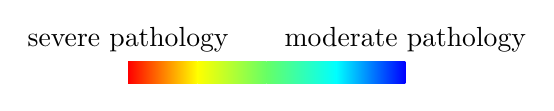
\begin{tikzpicture}[scale=\scalingFactor]
    \shade[left color=red,right color=yellow] (\gradLimLeft,2.5) rectangle (-0.8,2.75);
    \shade[left color=yellow,right color=barGreen] (-0.8,2.5) rectangle (0,2.75);
    \shade[left color=barGreen,right color=cyan] (0,2.5) rectangle (0.8,2.75);	
    \shade[left color=cyan,right color=blue] (0.8,2.5) rectangle (\gradLimRight,2.75);   

    \node[inner sep=0] (corr_text) at (\gradLimLeft,3) {severe pathology};
    \node[inner sep=0] (corr_text) at (\gradLimRight,3) {moderate pathology};
  \end{tikzpicture}
  \vspace{0.3em}
  \end{subfigure}
  

  
  \begin{subfigure}[b]{0.2 \textwidth}
   \centering
   \Large{ADNI MRI}
  \includegraphics[width=\textwidth,trim=0 0 0 20,clip]{\voxFld/selected_resfiles/adniThick/atrophyExtent24_adniThInitk-meansCl3Pr1Ra1_VDPM_MRF.png}
  \end{subfigure} 
  ~
  \begin{subfigure}[b]{0.2 \textwidth}
   \centering
   \Large{DRC tAD}
  \includegraphics[width=\textwidth,trim=0 0 0 20,clip]{\voxFld/selected_resfiles/drcAD/atrophyExtent24_drcThInitk-meansCl3Pr1Ra1_VDPM_MRFAD.png}
  \end{subfigure}
  \vspace{0.5em}

  \begin{subfigure}[b]{0.2 \textwidth}
   \centering
   \Large{DRC PCA}
  \includegraphics[width=\textwidth,trim=0 0 0 20,clip]{\voxFld/selected_resfiles/drcPCA/atrophyExtent24_drcThInitk-meansCl5Pr1Ra1_VDPM_MRFPCA.png}
  \end{subfigure}
  ~
  \begin{subfigure}[b]{0.2 \textwidth}
   \centering
   \Large{ADNI PET AV45}
  \includegraphics[width=\textwidth,trim=0 0 0 20,clip]{\voxFld/selected_resfiles/adniPet/atrophyExtent24_adniPetInitk-meansCl18Pr1Ra1_VDPM_MRF.png}
  \end{subfigure}
  
  \small{Marinescu et al., NeuroImage, 2019}\\
  %\small{source code: https://github.com/mrazvan22/dive}

\end{figure}


\end{frame}



% \begin{frame}
% \frametitle{DIVE Estimates the Temporal Evolution of Pathology, Enabling Understanding of Disease Mechanisms}
% 
% 
% \newcommand{\scalingFactor}{1.2}
% \newcommand{\gradLimLeft}{-1.6}
% \newcommand{\gradLimRight}{1.6}
% 
% \definecolor{barGreen}{rgb}{0.4,1,0.4}
% 
% \newcommand{\speed}{2}
% 
% \vfill
% 
% 
% % FWHM0 avg thickness map MCI & AD
% \begin{figure}[h]
%   \centering
%   \vspace{-1em}
% 
%   % do the legend colorbar
%   \begin{subfigure}[b]{0.45\textwidth}
%    \centering
%   \begin{tikzpicture}[scale=\scalingFactor]
%     \shade[left color=red,right color=yellow] (\gradLimLeft,2.5) rectangle (-0.8,2.75);
%     \shade[left color=yellow,right color=barGreen] (-0.8,2.5) rectangle (0,2.75);
%     \shade[left color=barGreen,right color=cyan] (0,2.5) rectangle (0.8,2.75);	
%     \shade[left color=cyan,right color=blue] (0.8,2.5) rectangle (\gradLimRight,2.75);   
% 
%     \node[inner sep=0] (corr_text) at (\gradLimLeft,3) {severe pathology};
%     \node[inner sep=0] (corr_text) at (\gradLimRight,3) {moderate pathology};
%   \end{tikzpicture}
%   \vspace{0.3em}
%   \end{subfigure}
%   
% 
% 	\begin{animateinline}[autoplay,loop]{\speed}  
%    \multiframe{20}{i=10+1}{% loop through pictures
% %  \multiframe{1}{i=10+1}{% loop through pictures \multiframe{nrOfPics}{i=initialVal+increment} 
%   
%   \parbox{\textwidth}{
%   \centering
%   
%   \begin{subfigure}[b]{0.25 \textwidth}
%    \centering
%    \Large{ADNI MRI}
%     \includegraphics[width=\textwidth]{\voxFld/selected_resfiles/adniThick/movie_adniThInitk-meansCl3Pr1Ra1_VDPM_MRFtext_\i}
%   \end{subfigure} 
%   ~
%   \begin{subfigure}[b]{0.25 \textwidth}
%    \centering
%    \Large{DRC tAD}
%   \includegraphics[width=\textwidth]{\voxFld/selected_resfiles/drcAD/movie_drcThInitk-meansCl3Pr1Ra1_VDPM_MRFADtext_\i}
%   \end{subfigure}
%   \vspace{0.5em}
% 
% 
%   \begin{subfigure}[b]{0.25 \textwidth}
%    \centering
%    \Large{DRC PCA}
%     \includegraphics[width=\textwidth]{\voxFld/selected_resfiles/drcPCA/movie_drcThInitk-meansCl5Pr1Ra1_VDPM_MRFPCAtext_\i} 
%   \end{subfigure}
%   ~
%   \begin{subfigure}[b]{0.25 \textwidth}
%    \centering
%    \Large{ADNI PET AV45}
%    \includegraphics[width=\textwidth]{\voxFld/selected_resfiles/adniPet/movie_adniPetInitk-meansCl18Pr1Ra1_VDPM_MRFtext_\i} 
%   \end{subfigure}
%   
%   }  
%   }
%   \end{animateinline}
% 
%   
%   \small{Marinescu et al., Neuroimage, 2019}\\
%   \small{source code: https://github.com/mrazvan22/dive}
% 
% \end{figure}
% 
% % \begin{itemize}
% %  \item Animations generated using BrainPainter: https://github.com/mrazvan22/brain-coloring
% % \end{itemize}
% 
% \end{frame}




%%%%%%%%%%%%%%%%%%%%%%%%%%%%%%%%%%%%%%%%%%%%%%%%%%%%%%%%%%%%%

% \newcommand{\ipmiPaperFold}{.}
\newcommand{\outFoldADNICVbrains}{../overview/figures_ipmi_paper/crossvalid/adniThavgFWHM0Initk-meansCl3Pr0Ra1_VWDPMMean}
\newcommand{\scaleFig}{0.19}

\begin{frame}
\frametitle{Validation - Model Robustly Estimates Atrophy Patterns}

\textbf{Method:} Tested the consistency of the spatial clustering in ADNI using 10-fold CV\\
\vspace{1em}

\textbf{Results:} Good agreement in terms of spatial distribution (dice score 0.89)\\

\begin{figure}[h]
    \centering
    
%     \newcounter{classnumber}
    \foreach \n in {1,...,5}{
    \begin{subfigure}[b]{\scaleFig\textwidth}
    \centering
    f=\n \\
    \includegraphics[width=\textwidth]{\outFoldADNICVbrains/blend\n.png}\\
%     \vspace{-1.5em}
    \includegraphics[width=\textwidth,trim=0 0 0 25,clip]{../overview/figures/cogCorr/trajSamplesOneFig_cogCorr_adniThFWHM0Initk-meansCl3Pr0Ra1Mrf5_VWDPMMean_f\n.png}
    \end{subfigure}
    }
    
%     \caption{Cross-validation}
    \label{fig:ADNICVbrains}
\end{figure}
\vspace{-2em}
\begin{center}
\small{Marinescu et al., Neuroimage, 2019}\\
%\small{source code: https://github.com/mrazvan22/dive}
\end{center}

\end{frame}

%%%%%%%%%%%%%%%%%%%%%%%%%%%%%%%%%%%%%%%%%%%%%%%%%%%%%%%%%%%%%

% \begin{frame}
% \frametitle{Estimated Subject Progression Scores are Clinically Relevant}
% 
% \vspace{-2em}
% 
% \textbf{Hypothesis}: 
% \begin{itemize}
%  \item Clinical relevance $\rightarrow$ DPS correlates with other markers of disease progression
% \end{itemize}
% 
% \vfill
% 
% \textbf{Method}: Ran our model on ADNI using 10-fold cross-validation
% 
% \vfill
% 
% \textbf{Results}: Progression scores correlate well with cognitive tests:
% 
% 
% 
% \newcommand{\figFont}{\small}
% \newcommand{\pValFont}{\tiny}
% 
% \begin{figure}[h]
%   \begin{subfigure}{0.22\textwidth}
%     \centering
%     \figFont{CDRSOB}\\ \pValFont{($\rho = 0.41$, $p < 1e-66$)}
%     \includegraphics[width=1.1\textwidth]{../overview/figures/stagingCogTestsScatterPlot_adniThFWHM0Initk-meansCl3Pr0Ra1Mrf5_VWDPMMean_ADAS13.png}
%   \end{subfigure}
%   \begin{subfigure}{0.22\textwidth}
%     \centering
%     \figFont{ADAS-COG}\\ \pValFont{($\rho = -0.40$, $p < 1e-62$)}
%     \includegraphics[width=1.1\textwidth]{../overview/figures/stagingCogTestsScatterPlot_adniThFWHM0Initk-meansCl3Pr0Ra1Mrf5_VWDPMMean_MMSE.png}
%   \end{subfigure}
%     \begin{subfigure}{0.22\textwidth}
%     \centering
%     \figFont{MMSE}\\ \pValFont{($\rho = -0.39$, $p < 1e-58$)}
%     \includegraphics[width=1.1\textwidth]{../overview/figures/stagingCogTestsScatterPlot_adniThFWHM0Initk-meansCl3Pr0Ra1Mrf5_VWDPMMean_RAVLT.png}
%   \end{subfigure}
%     \begin{subfigure}{0.22\textwidth}
%     \centering
%     \figFont{RAVLT}\\ \pValFont{($\rho = 0.39$, $p < 1e-58$)}
%     \includegraphics[width=1.1\textwidth]{../overview/figures/stagingCogTestsScatterPlot_adniThFWHM0Initk-meansCl3Pr0Ra1Mrf5_VWDPMMean_CDRSOB.png}
%   \end{subfigure}
% \end{figure}
% 
% \vspace{-2em}
% 
% 
% \end{frame}


\begin{frame}{Disease Progression Modelling -- Summary}

\begin{itemize}
 \item We modelled the continuous progression of Alzheimer's disease and related dementias
 
 \vo
 
 \item Used generative bayesian model that does not require labels (unsupervised)
 
 \vo
 
 \item However, such models require good quality data, to perform segmentation and extract disease markers
 
 \vo
 
 \item How can we do such modelling for scans with limited resolution and contrast?
\end{itemize}

 
\end{frame}


% \begin{frame}[label=current]
% \frametitle{Future research directions}
% 
% \textbf{Modelling}:
% \begin{itemize}
% \item Incorporate biological mechanisms (Raj et al., 2012,  Georgiadis et al., 2018)
% \item Incorporate other sources of data: e.g. genetics (Sclesi et al, Brain, 2018)
% \item Account for heterogeneity (e.g. Young et al., Nature Comm., 2018)
% \end{itemize}
% 
% \vfill
% 
% \textbf{Simulations}: 
% \begin{itemize}
% \item Use disease progression models to simulate cohorts (Koval et al., arXiv, 2019)
% \end{itemize}
% 
% \vfill
% 
% \textbf{Applications}:
% \begin{itemize}
% \item Other NDs: Multiple Sclerosis, Huntington's, Parkinson's
% \item Other pathologies: e.g. tumours, lesions
% \end{itemize}
% 
% \end{frame}


% \begin{frame}[label=current]
% \frametitle{BrainPainter features}
% 
% Brain types:
% \begin{figure}
% \centering
% 
% pial
% 
% 
% inflated
% 
% \end{figure}
% 
% 
% \end{frame}


% \begin{frame}[label=current]
% \frametitle{Acknowledgements}
% 
% % \includegraphics[width=\textwidth,trim=0 0 0 150, clip]{cmic_away_day}
%  
%  \begin{small}
% \begin{columns}[T]
% %     \hspace{-4em}
%     \begin{column}{.3\textwidth}
%     \textbf{Collaborators}
%     \begin{enumerate}
%     \item Leon Aksman
%     \item Maura Bellio
%      \item Arman Eshaghi
%      \item Nicholas Firth
%      \item Sara Garbarino
%      \item Marco Lorenzi
%      \item Kyriaki Mengoudi
%      \item Neil Oxtoby
%      \item Alexandra Young
%     \end{enumerate}
% %     \includegraphics[scale=1]{pondLogo.png}  
%     \end{column}
%     
%     
% %     \begin{column}{.6\textwidth}
% %     \begin{center}
% %     \textbf{Project Supervisors}
% %     \end{center}
% %     \vspace{-2em}
% %       \begin{figure}
% %       \begin{subfigure}{0.3\textwidth}
% %       \centering
% %       Daniel Alexander
% %       \includegraphics[height=2cm]{Danny-Alexander.jpeg}  
% %       \end{subfigure}
% % 	\begin{subfigure}{0.3\textwidth}
% % 	\centering
% %       Sebastian Crutch
% %       \includegraphics[height=2cm]{Seb_Crutch_photo.JPG}  
% %       \end{subfigure}
% %   \begin{subfigure}{0.3\textwidth}
% % 	\centering
% %       Polina Golland
% %       \includegraphics[height=2cm, trim=0 00 0 0,clip]{polina}  
% %       \end{subfigure}
% %       
% %     \begin{center}
% %     \textbf{Funders}
% %     \end{center}
% %     %\vspace{-2em}
% %       \begin{subfigure}{0.3\textwidth}
% %       \centering
% %       \includegraphics[height=1cm]{epsrc_logo}  
% %       \end{subfigure}
% % 	\begin{subfigure}{0.3\textwidth}
% % 	\centering
% %       \includegraphics[height=1cm]{CDTlogo}  
% %       \end{subfigure}
% %      
% %       
% %       \vspace{2em}
% % 
% % \end{figure}
% %     
% % \end{column}
% \end{columns}
%  
% \end{small}
% 
% 
% \end{frame}

